\documentclass[a4paper,12pt]{article}
\usepackage{pdflscape, float, graphicx, color, listings, color}
\usepackage[top=1.5cm, bottom=1.6cm, left=2.0cm, right=2.0cm]{geometry}
\usepackage[dvipsnames]{xcolor}
\title{CS22510 Assignment 1\\
Runners and Riders\\
"Out and About"}
\author{Chris Savill\\\texttt{chs17@aber.ac.uk}}

\lstdefinestyle{customc++} {
  belowcaptionskip=1\baselineskip,
  breaklines=true,
  frame=L,
  language=C++,
  showstringspaces=false,
  basicstyle=\footnotesize\ttfamily,
  keywordstyle=\bfseries\color{OliveGreen},
  commentstyle=\itshape\color{black},
  identifierstyle=\color{blue},
  stringstyle=\color{orange},
  numbers=left
}

\lstdefinestyle{customjava} {
  belowcaptionskip=1\baselineskip,
  breaklines=true,
  frame=L,
  language=Java,
  showstringspaces=false,
  basicstyle=\footnotesize\ttfamily,
  keywordstyle=\bfseries\color{blue},
  commentstyle=\itshape\color{black},
  identifierstyle=\color{OliveGreen},
  stringstyle=\color{orange},
  numbers=left
}


\begin{document}
\maketitle
\newpage
\tableofcontents
\newpage

\section{Description of three programs}

\subsection{Event Creation Program}

\subsection{Checkpoint Manager Program}

\subsection{Event Manager Program}

\section{Code for the Event Creation Program}
\subsection{Header files}
\lstinputlisting[style=customc++, label={creator.h}, caption=Header file for non-class specific functions.]{"/home/clsavill/GitHub/Runners_and_Riders_3_Part/Event_Creation_Program/creator.h"}
\lstinputlisting[style=customc++, label={event.h}, caption=Header file Event class.]{/home/clsavill/GitHub/Runners_and_Riders_3_Part/Event_Creation_Program/event.h}
\lstinputlisting[style=customc++, label={course.h}, caption=Header file for Course class.]{/home/clsavill/GitHub/Runners_and_Riders_3_Part/Event_Creation_Program/course.h}
\lstinputlisting[style=customc++, label={competitor.h}, caption=Header file for Competitor class.]{/home/clsavill/GitHub/Runners_and_Riders_3_Part/Event_Creation_Program/competitor.h}

\subsection{Cpp files}
\lstinputlisting[style=customc++, label={creator.cpp}, caption=Main method and menu file.]{/home/clsavill/GitHub/Runners_and_Riders_3_Part/Event_Creation_Program/main.cpp}
\lstinputlisting[style=customc++, label={event.cpp}, caption=Cpp file for Event class.]{/home/clsavill/GitHub/Runners_and_Riders_3_Part/Event_Creation_Program/event.cpp}
\lstinputlisting[style=customc++, label={course.cpp}, caption=Cpp file for Course class.]{/home/clsavill/GitHub/Runners_and_Riders_3_Part/Event_Creation_Program/course.cpp}
\lstinputlisting[style=customc++, label={competitor.cpp}, caption=Cpp file for Competitor class.]{/home/clsavill/GitHub/Runners_and_Riders_3_Part/Event_Creation_Program/competitor.cpp}

\section{Clean build and compilation of Event Creation Program}
\lstinputlisting[breaklines=true, basicstyle=\footnotesize\ttfamily]{/home/clsavill/GitHub/Runners_and_Riders_3_Part/Event_Creation_Program/Event_Creation_Clean_And_Build_Log.txt}

\section{Run through of Event Creation Program}
\lstinputlisting[breaklines=true, basicstyle=\footnotesize\ttfamily]{/home/clsavill/GitHub/Runners_and_Riders_3_Part/Event_Creation_Program/Event_Creation_Runthrough.txt}

\section{Files created by execution of Event Creation Program}
\lstinputlisting[breaklines=true, basicstyle=\footnotesize\ttfamily, caption=Event 'name.txt' file]
{/home/clsavill/GitHub/Runners_and_Riders_3_Part/Event_Creation_Program/name.txt}

\lstinputlisting[breaklines=true, basicstyle=\footnotesize\ttfamily, caption=Event 'courses.txt' file]
{/home/clsavill/GitHub/Runners_and_Riders_3_Part/Event_Creation_Program/courses.txt}

\lstinputlisting[breaklines=true, basicstyle=\footnotesize\ttfamily, caption=Event 'entrants.txt' file]
{/home/clsavill/GitHub/Runners_and_Riders_3_Part/Event_Creation_Program/entrants.txt}

\section{Code for Checkpoint Manager Program}
\lstinputlisting[style=customjava, label={Launcher.java}, caption=Launcher class.]{/home/clsavill/GitHub/Runners_and_Riders_3_Part/Checkpoint_Manager_Program/src/Data_Structures/Launcher.java}
\lstinputlisting[style=customjava, label={Event.java}, caption=Event class.]{/home/clsavill/GitHub/Runners_and_Riders_3_Part/Checkpoint_Manager_Program/src/Data_Structures/Event.java}
\lstinputlisting[style=customjava, label={Node.java}, caption=Node class.]{/home/clsavill/GitHub/Runners_and_Riders_3_Part/Checkpoint_Manager_Program/src/Data_Structures/Node.java}
\lstinputlisting[style=customjava, label={Course.java}, caption=Course class.]{/home/clsavill/GitHub/Runners_and_Riders_3_Part/Checkpoint_Manager_Program/src/Data_Structures/Course.java}
\lstinputlisting[style=customjava, label={Competitor.java}, caption=Competitor class.]{/home/clsavill/GitHub/Runners_and_Riders_3_Part/Checkpoint_Manager_Program/src/Data_Structures/Competitor.java}
\lstinputlisting[style=customjava, label={Record.java}, caption=Record class.]{/home/clsavill/GitHub/Runners_and_Riders_3_Part/Checkpoint_Manager_Program/src/Data_Structures/Record.java}
\lstinputlisting[style=customjava, label={FileHandler.java}, caption=FileHandler class.]{/home/clsavill/GitHub/Runners_and_Riders_3_Part/Checkpoint_Manager_Program/src/File_Handling/FileHandler.java}
\lstinputlisting[style=customjava, label={TypeWindow.java}, caption=TypeWindow class.]{/home/clsavill/GitHub/Runners_and_Riders_3_Part/Checkpoint_Manager_Program/src/GUI/TypeWindow.java}
\lstinputlisting[style=customjava, label={SelectionWindow.java}, caption=SelectionWindow class.]{/home/clsavill/GitHub/Runners_and_Riders_3_Part/Checkpoint_Manager_Program/src/GUI/SelectionWindow.java}
\lstinputlisting[style=customjava, label={TimeWindow.java}, caption=TimeWindow class.]{/home/clsavill/GitHub/Runners_and_Riders_3_Part/Checkpoint_Manager_Program/src/GUI/TimeWindow.java}

\section{Clean build and compilation of Checkpoint Program}
\lstinputlisting[breaklines=true, basicstyle=\footnotesize\ttfamily]{/home/clsavill/GitHub/Runners_and_Riders_3_Part/Checkpoint_Manager_Program/Checkpoint_Manager_Clean_And_Build_Log.txt}

\section{Run through of Checkpoint Manager Program}
\begin{figure}[H]
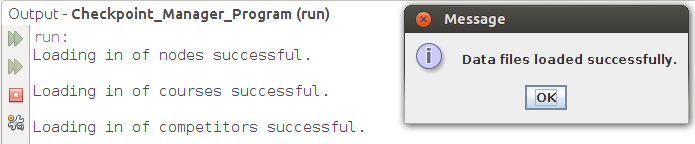
\includegraphics[scale=0.8]{/home/clsavill/GitHub/Runners_and_Riders_3_Part/Checkpoint_Manager_Program/CMP1.png}
\caption{Start up of GUI letting user know data file loaded successfully ( if they did) else the program would close.}
\end{figure}

\begin{figure}[H]
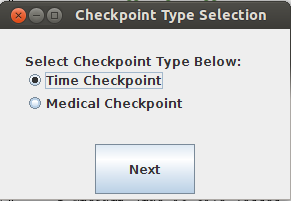
\includegraphics[scale=0.8]{/home/clsavill/GitHub/Runners_and_Riders_3_Part/Checkpoint_Manager_Program/CMP2.png}
\caption{Checkpoint type selection window showing the time checkpoint type selected.}
\end{figure}

\begin{figure}[H]
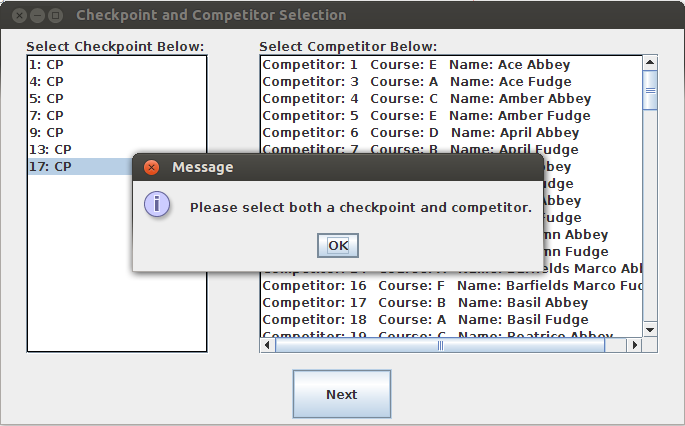
\includegraphics[scale=0.8]{/home/clsavill/GitHub/Runners_and_Riders_3_Part/Checkpoint_Manager_Program/CMP3.png}
\caption{Message that pops up when both a checkpoint and competitor are not selected.}
\end{figure}

\begin{figure}[H]
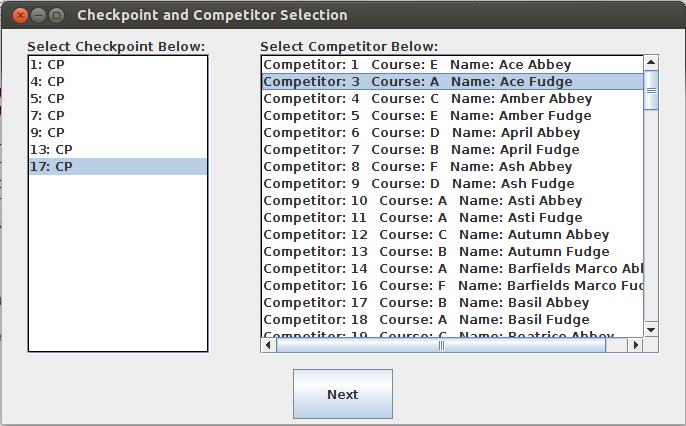
\includegraphics[scale=0.8]{/home/clsavill/GitHub/Runners_and_Riders_3_Part/Checkpoint_Manager_Program/CMP4.png}
\caption{Time checkpoint 17 selection and competitor 3 selected within selection window.}
\end{figure}

\begin{figure}[H]
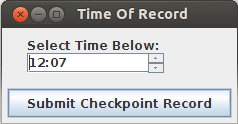
\includegraphics[scale=0.8]{/home/clsavill/GitHub/Runners_and_Riders_3_Part/Checkpoint_Manager_Program/CMP5.png}
\caption{Time window where the user has to input the time for the new record.}
\end{figure}

\begin{figure}[H]
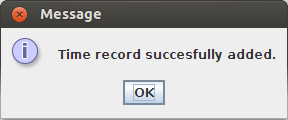
\includegraphics[scale=0.8]{/home/clsavill/GitHub/Runners_and_Riders_3_Part/Checkpoint_Manager_Program/CMP6.png}
\caption{Message stating that the new record was successfully added and written to the time records file.}
\end{figure}

\begin{figure}[H]
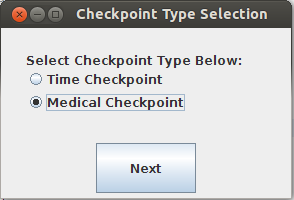
\includegraphics[scale=0.8]{/home/clsavill/GitHub/Runners_and_Riders_3_Part/Checkpoint_Manager_Program/CMP7.png}
\caption{Checkpoint type selection window showing the medical checkpoint type selected.}
\end{figure}

\begin{figure}[H]
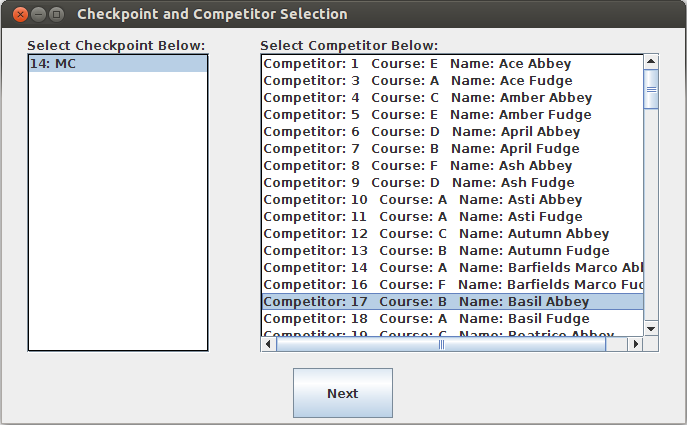
\includegraphics[scale=0.8]{/home/clsavill/GitHub/Runners_and_Riders_3_Part/Checkpoint_Manager_Program/CMP8.png}
\caption{Medical checkpoint 14 selection and competitor 17 selected within the selection window.}
\end{figure}

\begin{figure}[H]

\includegraphics[scale=0.8]{/home/clsavill/GitHub/Runners_and_Riders_3_Part/Checkpoint_Manager_Program/CMP9.png}
\caption{Prompt asking the user the status of the competitor at the chosen medical checkpoint.}
\end{figure}

\begin{figure}[H]
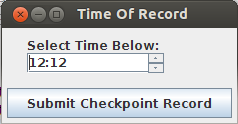
\includegraphics[scale=0.8]{/home/clsavill/GitHub/Runners_and_Riders_3_Part/Checkpoint_Manager_Program/CMP10.png}
\caption{Time window with a valid time entered (a time after the last record time.}
\end{figure}

\begin{figure}[H]
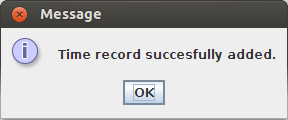
\includegraphics[scale=0.8]{/home/clsavill/GitHub/Runners_and_Riders_3_Part/Checkpoint_Manager_Program/CMP6.png}
\caption{Message stating that the new record was successfully added and written to the time records file.}
\end{figure}

\begin{figure}[H]
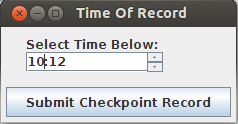
\includegraphics[scale=0.8]{/home/clsavill/GitHub/Runners_and_Riders_3_Part/Checkpoint_Manager_Program/CMP11.png}
\caption{The same record as above time window with an invalid time entered (a time before the last record time.}
\end{figure}

\begin{figure}[H]

\includegraphics[scale=0.8]{/home/clsavill/GitHub/Runners_and_Riders_3_Part/Checkpoint_Manager_Program/CMP12.png}
\caption{Message stating that the new record attempted to be added was invalid (either the time was before the last record, or the system determined that the status given cannot be correct due to the current status of the competitor.}
\end{figure}

\section{Files created by execution of Checkpoint Manager\\Program}
\lstinputlisting[breaklines=true, basicstyle=\footnotesize\ttfamily, caption=Copy of cp\_times\_1.txt file from event\_3 that was read into the program plus 2 new records appended.]{/home/clsavill/GitHub/Runners_and_Riders_3_Part/Checkpoint_Manager_Program/cp_times.txt}

\section{Clean build and compilation of Event Manager Program}
\lstinputlisting[breaklines=true, basicstyle=\footnotesize\ttfamily]{/home/clsavill/GitHub/Runners_and_Riders_3_Part/Event_Manager_Program/Event_Manager_Clean_And_Build_Log.txt}

\begin{landscape}
\section{Run through of Event Manager Program}
\lstinputlisting[breaklines=true, basicstyle=\footnotesize\ttfamily]{/home/clsavill/GitHub/Runners_and_Riders_3_Part/Event_Manager_Program/Event_Manager_Runthrough.txt}

\section{Results list produced at the end of an event}

\subsection{Results of successful competitors}
\lstinputlisting[breaklines=true, basicstyle=\footnotesize\ttfamily]{/home/clsavill/GitHub/Runners_and_Riders_3_Part/Event_Manager_Program/Event_Manager_Results.txt}

\subsection{Table of excluded competitors}
\lstinputlisting[breaklines=true, basicstyle=\footnotesize\ttfamily]{/home/clsavill/GitHub/Runners_and_Riders_3_Part/Event_Manager_Program/Event_Manager_Excluded.txt}

\section{Log file contents}
\lstinputlisting[breaklines=true, basicstyle=\footnotesize\ttfamily]{/home/clsavill/GitHub/Runners_and_Riders_3_Part/Event_Manager_Program/log.txt}

\end{landscape}

\end{document}